\documentclass[10pt]{article}
\usepackage{parskip}
\usepackage[utf8]{inputenc}
\usepackage[left=2.00cm, right=2.00cm, top=2.00cm, bottom=2.00cm]{geometry}
\usepackage[spanish]{babel}
\usepackage{graphicx,subfig}
\usepackage{fancyhdr}
\usepackage{pgfplots}
\graphicspath{{Imagenes/}}
\usepackage{enumerate} 
\usepackage{multicol}
\usepackage{tabularx}
\usepackage{amssymb}
\usepackage{adjustbox}
\usepackage{amsmath}
\usepackage{cancel}
\begin{document}


\pagestyle{fancy}
\cfoot{}


%Cabeceras
\rhead{Péndulo Simple.}
\lhead{}

%Portada
\begin{titlepage}
	\newgeometry{
		left=25mm,
		right=25mm,
		top=5mm,
		bottom=30mm,
		headheight = 0 mm
	}

	\begin{figure}[t]
		\subfloat{
\includegraphics[width=0.15\textwidth]{Logo_IPN}}
		\hspace{0.6\textwidth}
		\subfloat{
\includegraphics[width=0.22\textwidth]{LogoEsime}}
	\end{figure}

	\centering
	{\bfseries\Huge Instituto Politécnico Nacional. \par}
	\vspace{1cm}
	{\scshape\Large Ingeniería en Comunicaciones y Electrónica. \par}
	\vspace{0.3cm}
	{\scshape\Large Laboratorio de Electricidad y Magnetismo.  \par}
	\vspace{1cm}
	{\scshape\Huge ¡MUEVASE O ME LO LLEVO! \par}
	\vspace{1cm}
	{\itshape\Large Pendulo simple \par}
	{\Large 2CM13\par}
	\vfill
	
	{\Large  \par}
	{\Large   \par}
	{\Large  \par}
	{\Large \par}
	{\Large   \par}
	{\Large \par}
	\vfill
	{\Large Octubre 2023. \par}

\end{titlepage}

\tableofcontents
\newpage
\begin{center}
	Hernández Huerta Jose Emilio, 
	Hernández Sanluis Danna Estefany,  
	Garduño Bejarano Nataly,
	Mojica Reyes Rogelio,
	Morlan Juárez Bruno Tonatiuh,  
	Santos Marañón María Renée.
\end{center}

\section{Resumen.}
Este informe de laboratorio se enfoca en el estudio de un péndulo simple y su comportamiento en relación con diferentes variables. El experimento se divide en tres partes principales: la influencia de la amplitud en el periodo, la influencia de la masa en el periodo y la relación entre la longitud de la cuerda y el periodo del péndulo. A través de experimentos cuidadosamente diseñados y mediciones precisas, se ha demostrado que la amplitud y la masa no afectan significativamente el periodo del péndulo simple, mientras que la longitud de la cuerda tiene una influencia directa en el periodo, siguiendo una relación teórica bien establecida. Además, se ha calculado el valor de la gravedad local utilizando los resultados experimentales. Este informe proporciona una comprensión sólida de los principios fundamentales del péndulo simple y demuestra la importancia de las variables en su comportamiento. También se ha realizado un análisis estadístico para evaluar la precisión de las mediciones y estimar la incertidumbre en los resultados.

\begin{multicols}{2}

\section{Objetivo.}
A través de esta práctica se determinar como influye en el periodo de oscilación de un péndulo simple  , la amplitud de oscilación , la masa del péndulo , la longitud del péndulo simple y obtener el valor numérico de la aceleración de la gravedad midiendo el periodo y la longitud del péndulo simple .



\section{Marco teórico.}
Un péndulo simple es un sistema mecánico, constituido por una masa puntual, suspendida de un hilo inextensible y sin peso. Cuando se separa hacia un lado de su posición de equilibrio y se le suelta, el péndulo oscila en un plano vertical bajo la influencia de la gravedad. El movimiento es periódico y oscilatorio. Si un pequeño cuerpo de masa m se encuentra sujeto al extremo de un hilo de peso despreciable, cuya longitud es L y que oscila en un plano vertical. Este dispositivo constituye un Péndulo Simple en oscilación, herramienta muy importante en los trabajos realizados por Galileo, Newton y Huygens.
\begin{center}
	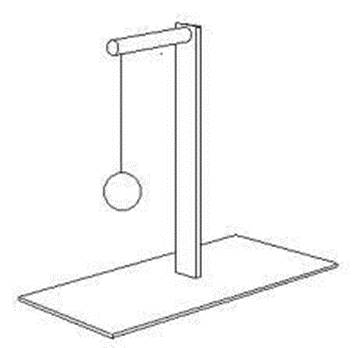
\includegraphics[width=4cm, height=7cm]{Imagenes/pendulo.png}
	\captionof{figure}{Pendulo Simple.}
	\label{fig:es}
\end{center}
Posteriormente surgió el llamado péndulo de Foucault es un péndulo largo que se puede oscilar libremente en cualquier plano vertical y capas de oscilar durante horas .Se utiliza para demostrar la rotación de la Tierra . Fig \ref{fig:es}
En el péndulo más sencillo, el llamado péndulo simple, puede considerarse que
toda la masa del dispositivo está concentrada en un punto del objeto oscilante, y
dicho punto sólo se mueve en un plano. El movimiento del péndulo de un reloj se
aproxima bastante al de un péndulo simple. El péndulo esférico, en cambio, no
está limitado a oscilar en un 
El péndulo mas sencillo , es llamado péndulo simple , puede considerarse que toda la masa del dispositivo esta conectada en un punto del objeto oscilante y dicho punto solo se mueve en un plano . El movimiento del péndulo de un reloj se aproxima bastante al de un péndulo simple .El péndulo esférico , en cambio no esta limitado a oscilar en un único plano , por lo que su movimiento es mucho màs complejo . 
Sin embargo , como el movimiento del péndulo depende de la gravedad , su periodo varia con la localización geográfica , puesto que la gravedad es mas o menos intensa según la latitud y altitud , Por ejemplo el periodo de un  péndulo dado será mayor en una montaña que a nivel del mar . por eso un péndulo simple permite determinar con `precisión la aceleración local de la gravedad .
\begin{itemize}
	\item Longitud del Péndulo y Periodo:
\end{itemize}
 La longitud del péndulo simple tiene una influencia directa en su período. Cuanto mayor sea la longitud, mayor será el período, y viceversa. Esta relación se expresa en la fórmula $\tau = 2\pi \sqrt{\frac{L}{g}}$, donde "L" es la longitud y "g" es la aceleración debida a la gravedad. Fig \ref{fig:pendulo y periodo}

 \begin{center}
	\includegraphics[width=7cm, height=4cm]{Imagenes/Longitud del Péndulo y Periodo.png}
	\captionof{figure}{Pendulo y Periodo.}
	\label{fig:pendulo y periodo}
\end{center}
\begin{itemize}
	\item Ecuación del Péndulo Simple:
\end{itemize}
La ecuación que describe el movimiento de un péndulo simple es una ecuación diferencial no lineal que depende de la longitud del péndulo (L), la aceleración debido a la gravedad (g) y el ángulo de desplazamiento ($\theta$). Para pequeños ángulos de desplazamiento, el péndulo simple puede describirse aproximadamente mediante la ecuación del movimiento armónico simple: $\theta = \theta_{0} $* cos($\omega$t), donde $\theta_0$ es la amplitud y $\omega$ es la frecuencia angular.

\begin{itemize}
	\item Movimiento Armónico Simple (MAS): 
\end{itemize}
El péndulo simple se comporta como un ejemplo de movimiento armónico simple. El MAS es un movimiento periódico y oscilatorio en torno a una posición de equilibrio estable. En el caso del péndulo simple, este movimiento es aproximadamente sinusoidal. Fig \ref{fig:mas}

\begin{center}
	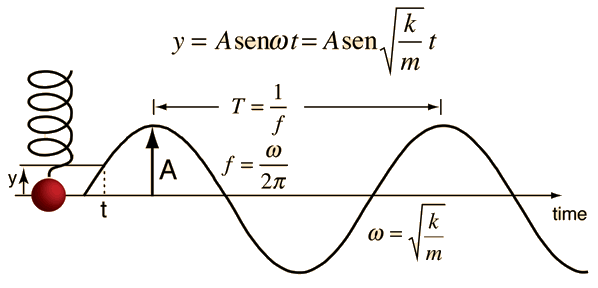
\includegraphics[width=7cm, height=4cm]{Imagenes/mas.png}
	\captionof{figure}{Movimiento Armonico Simple.}
	\label{fig:mas}
\end{center}

\begin{itemize}
	\item Período y Frecuencia:
\end{itemize}
El período de un péndulo simple es el tiempo que tarda en realizar una oscilación completa, y se representa como "T". La frecuencia, representada como "f", es el número de oscilaciones completas que realiza el péndulo en un segundo y se calcula como el inverso del período (f = 1 / T). Fig \ref{fig:pe}

\begin{center}
	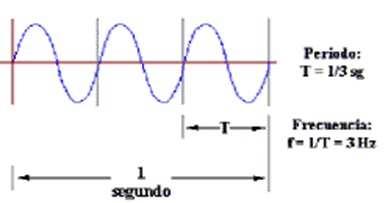
\includegraphics[width=7cm, height=4cm]{Imagenes/periodo.png}
	\captionof{figure}{Periodo y Frecuencia.}
	\label{fig:pe}
\end{center}


Materiales .-
1 Transportador .
1 Calibrador vernier.
1 Cronometro.
1 Flexómetro .
1 Péndulo con hilo cáñamo con masa pequeña .
1 Péndulo con hilo cáñamo con masa pesada .

\section{Experimento No.1- Influencia de la amplitud de oscilación en el periodo de un péndulo}
 

\begin{center}
	\begin{adjustbox}{width=245pt}
		\begin{tabular}{|c|c|c|c|c|c|c|c|c|c|c|c|}
			\hline
			&\multicolumn{6}{|c|}{Ampliruddes Pequeñas} & \multicolumn{5}{|c|}{Ampliruddes Grandes}\\
			\hline
			$\theta$ & 2 & 3 & 4 & 5 & 6 & 10 & 20 & 30 & 40 & 50 & 60 \\
			\hline
			t(s) & 27.7&	27.78&	27.96&	27.34&	27.03	&26.24&	27.3	&27.62	&27.82&	27.92&	27.38 \\
			\hline
			T(s) &1.385&	1.389&	1.398	&1.367&	1.3515&	1.312&	1.365&	1.381	&1.391	&1.396	&1.369
			\\
			\hline
			
		\end{tabular}
	\end{adjustbox}
\end{center}


\begin{tikzpicture}
	\begin{axis}[
		xlabel={$t[s]$},
		ylabel={$T[s]$},
		axis lines=left,
		xmin=26.0, xmax=28.0,
		ymin=1.3, ymax=1.4,
		xtick={26.0,26.5,...,28.0},
		ytick={1.3,1.35,1.4},
		grid=both,
	]
	
	% Puntos de datos
	\addplot [black, mark=*] coordinates {
		(27.7, 1.385)
		(27.78, 1.389)
		(27.96, 1.398)
		(27.34, 1.367)
		(27.03, 1.3515)
		(26.24, 1.312)
		(27.3, 1.365)
		(27.62, 1.381)
		(27.82, 1.391)
		(27.92, 1.396)
		(27.38, 1.369)
	};
	\addplot [red, domain=26.0:28.0] {0.05*x };
	\node [red, above right] at (axis cs: 27, 1.33) {$y = 0.05x$};
	\end{axis}
	\end{tikzpicture}

	¿el periodo de T se mantiene constante para todos los ángulos? 
	Si, ya que todas las oscilaciones se mantienen con una constante de 1.3 y solo varean por centenas de numero 
	De acuerdo a los resultados en la tabla I, diga si influye $\theta$ en el periodo del péndulo 
	No influye, ya que el periodo de las ondas es variable solo por centésimas de segundo
\section{Experimento No.2- Influencia de la masa}
Procedimiento Experimental:
Para esta sección de la practica usamos el mismo sistema que el del experimento 1, pero tuvimos que dejar dos situaciones constantes, en este caso fueron la longitud del péndulo (L), y la amplitud de oscilación ($\theta$). Los anteriores valores se mantuvieron en \\
L = 1 \\
$\theta = 2^{\circ}$ \\

Por lo que el sistema nos quedó de la siguiente manera: \\
\begin{center}
	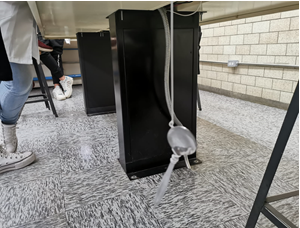
\includegraphics[width=4cm,height=5cm]{Imagenes/Masal.png}
	\captionof{figure}{Imagen de muestra como quedo el sistema de péndulo con la masa ligera (cuchara),a un metro de longitud de la cuerda del experimento.}
	\label{fig:1}
\end{center}

\begin{center}
	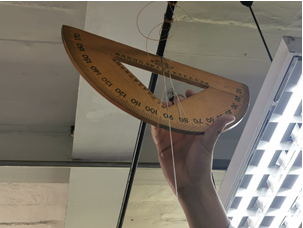
\includegraphics[width=4cm,height=5cm]{Imagenes/regla.png}
	\captionof{figure}{imagen de documentación sobre la medida contante que se tomó en cuanta, en cada oscilación, por lo menos en este experimento.}
	\label{fig:2}
\end{center}
Como se pudo observar no existía mayor problema en montar el sistema y ponerlo a oscilar, por lo que después de montar el experimento y ponerlo a oscilar 3 repeticiones, procedimos a medir cronometrar los tiempos de oscilación. Fig \ref{fig:1}
Si se puede resaltar algo de la dinámica de este experimento, es que por motivos de practicidad y de empezar tarde el experimento, para optimizar el tiempo medimos el tiempo de 10 oscilaciones con tres cronómetros diferentes y posteriormente calculamos el promedio de los antes mencionados. Fig \ref{fig:2}


\begin{center}
	\begin{adjustbox}{width=154pt}
		\begin{tabular}{|c|c|c|}
			\hline
			&Pesada &Ligera \\
			\hline
			$T_{1}$ &27.50&	25.77\\
			\hline
			$T_{2}$ &27.49&	25.74 \\
			\hline
			$T_{3}$ &26.77&	25.73 \\
			\hline
			$T_{1} \& T_{2}$ &27.25 s	&25.5 s\\
			\hline
		\end{tabular}
	\end{adjustbox}
\end{center}

Desarrollo Experimental:
Para determinar si la masa de los objetos afecta al periodo del péndulo lo primero que hicimos después de las mediciones, fue calcular su periodo, esto teniendo una relación entre el tiempo que se tardó cada una sobre el número de oscilaciones que se ejecutaron. \\
$\delta T_{1}=\frac{t_{1}}{n}=\frac{27.25}{10}=2.725 s$ \\ 
$\delta T_{2}=t_2/n=25.5/10=2.5756 s$ \\
Posteriormente determinamos el rango mínimo del cronometro y calculamos \\
$\delta_{t}=\frac{1}{100}=0.01 s$ \\
Se usará ese rango mínimo para los dos ya que ambas mediciones se hicieron con el mismo cronometro. \\
$\delta \tau=\frac{0.01}{10}=0.001s$\\
Después ingresamos todos nuestros datos en la tabla II, esto con el fin de llegar a un resultado

\begin{center}
	\begin{adjustbox}{width=245pt}
		\begin{tabular}{|c|c|c|c|c|}
			\hline
			Esfera	&t [s]	&T=t/n[s]&	$\delta t[s]$	&$\delta T= \frac{\delta t}{n}[s]$\\
			\hline
			No. 1 (pesada)&	27.25	&2.7255&	0.01	&0.001 \\
			\hline
			No.2 (ligera)&	25.5&	2.5756&	0.01&	0.001 \\
			\hline
		\end{tabular}
	\end{adjustbox}
\end{center}
Resultados: 
Nos quedaron como resultado de los dos objetos:\\
Masa 1:$ T_{1}^{*}=T_{1}\pm \delta T_{1}=2.7255\pm 0.001 s $\\
Masa 2: $T_{2}^{*}=T_{2}\pm \delta T_{2}=2.5756\pm 0.001 s $\\
Discusión: 
Al cambiar las masas:
- ¿Variamos la masa del péndulo?
Sí, porque, aunque la masa del péndulo no se considera de gran manera la masa del hilo, en este caso casi todo lo que contribuye al aspecto de la masa en este péndulo recae sobre la masa que posee cada masa, y por eso al cambiar de objeto también variamos a la masa del sistema.
- ¿Varía el periodo o se mantuvo constante?
Si tiene cierta variación, pero lo anterior está justificado por el hecho de que no estamos ante un sistema ideal, en el que no se aprecian tanto otros atributos de nuestro entorno (como la fricción del aire o la misma masa de la cuerda).
Pero en realidad no existe una variación extrema en el periodo, esto por el intervalo tan corto que se le dio a la oscilación al momento de accionarla.


El objetivo de este experimento era demostrar la independencia de la masa con respecto al periodo de oscilación, después de un arduo y preciso experimento determinamos que la masa no influye en el periodo de oscilación, no importando la magnitud que tenga la masa. Esto implica que un péndulo simple con un objeto pesado y otro con un objeto liviano, pero con la misma longitud de cuerda, tendrán el mismo periodo de oscilación.
Es importante destacar que esta relación es válida siempre y cuando las amplitudes de oscilación sean pequeñas, de manera que el movimiento pueda considerarse armónico simple.

\section{Experimento No.3- Relación entre la longitud y el periodo de un péndulo simple.}
Para este experimento con nuestra cuerda y un objeto de masa considerable (pedazo de imán), atamos la cuerda en una zona elevada aumentando su tamaño hasta llegar los 2 m, después, sujetamos el imán con la cuerda hasta una longitud de 0.80 m creando así un péndulo simple. Fig \ref{fig:pem}

\begin{center}
	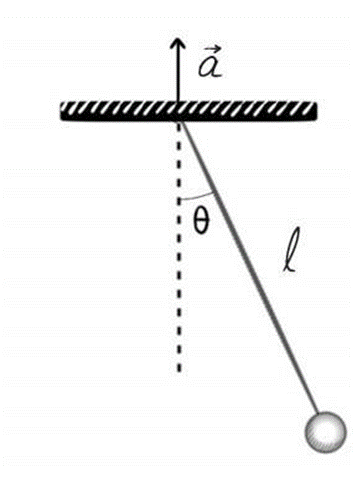
\includegraphics[width=4cm,height=5cm]{Imagenes/pemdulo.png}
	\captionof{figure}{Imagen de referencia a un péndulo simple.}
	\label{fig:pem}
\end{center}


Después de colocar nuestro sistema de referencia experimental, procedimos a contar 20 oscilaciones con una inclinación de 10° (se contaron a partir de las 3 primeras oscilaciones), el periodo se contó con el cronometro de 3 compañeros para obtener el resultado más preciso. 
Obtuvimos: 

\begin{center}
	\begin{adjustbox}{width=80pt}
		\begin{tabular}{|c|c|}
			\hline
			L[m] &T[s] \\
			\hline
			1	&19.59\\
			\hline
			0.80&	17.23\\
			\hline
			0.60 &	15.36\\
			\hline
			0.40&	13.18\\
			\hline
			0.25&	10.77\\
			\hline
		\end{tabular}
	\end{adjustbox}
\end{center}
Para comprobar si nuestros datos son acertados ocupamos a formula del periodo que es \\

$\tau = 2\pi \sqrt{\frac{L}{g}}$ \\

Sustituyendo nuestros valores iniciales para calcular el periodo de forma teórica obtuvimos
$\tau = 2\pi \sqrt{\frac{1m}{9.78 m/s^2 }}$\\
T= 2.009x10 ocilaciones\\
T= 20.09s\\
$\tau = 2\pi\sqrt{\frac{0.8m}{9.78 m/s^2}}$\\
T=1.79s x 10\\
= 17.9s\\
$\tau = 2\pi \sqrt{\frac{0.6m}{9.78 m/s^2}}$\\
T=1.55s x 10\\
= 15.5s\\
$\tau = 2\pi \sqrt{\frac{0.40m}{9.78 m/s^2}}$\\
T=1.27sx10\\
= 12.7s\\
$\tau = 2\pi \frac{0.25m}{9.78 m/s^2 }$\\
T=1.004sx10\\
=10.04s \\
Por lo que, nuestros valores se acercan al valor experimentado, concluimos con respecto a los demás experimentos que la distancia del laso ocupado durante un péndulo simple altera nuestro periodo, pues al notar que no está dentro de la ecuación $T= 2\pi \sqrt{\frac{L}{g}}$ no altera el sistema. 
Las incertidumbres de nuestros datos obtenidos son: 
Para el periodo la ecuación de la incertidumbre es: \\

$\delta T=\delta \frac{t}{n}=\frac{rango minimo del cronometro}{10}(s)$
Sustituyendo valores \\
El rango del cronometro va de $\frac{1}{1000}$ \\
$\delta T=\delta \frac{t}{n}= \frac{\frac{1}{100}}{10}$\\
$\delta T=1x10^{-3}$\\

Y para la longitud es: \\
$\delta L=\frac{1}{2}  rango minimo del flexometro(m)$\\
$\delta L=  \frac{1}{2} 0.01m$\\
$\delta L=\frac{1}{20}=0.05m $\\
Posterior a nuestra tabulación del experimento, se realizó una gráfica con la distancia de nuestra cuerda con respecto al periodo. 


\begin{tikzpicture}
	\begin{axis}[
		title={Grafica 2},
		xlabel={$L[m]$},
    	ylabel={$T[s]$},
		axis lines=left,
		xmin=0, xmax=1.2,
		ymin=0, ymax=20,
		xtick={0,0.2,0.4,0.6,0.8,1},
		ytick={0,5,10,15,20},
		grid=both,
	]
	
	% Puntos de datos
	\addplot [black, mark=*] coordinates {
		(1, 19.59)
		(0.8, 17.23)
		(0.6, 15.36)
		(0.4, 13.18)
		(0.25, 10.77)
	};
	\addplot [red, domain=26.0:28.0] { 11.368*x + 8.2915
	};
	\node [red, above right] at (axis cs: 0.4, 5) {$y = 11.368x + 8.2915$};
	\end{axis}
	\end{tikzpicture}
	
	Obteniendo nuestra grafica es recta, entonces, sabemos que es una función del tipo $Y=Ax^m$ por lo cual $L=AT^m $ \\
	Encontrando los valores de m partimos de la ecuación 
	Para calcular m sabemos que \\
	$m=\frac{h}{m}$
	Donde h es la altura de nuestra y b es la base de nuestra grafica 
	Sustituyendo los datos obtenemos que \\
	
	m=$\frac{19.59cm}{15.2cm}$ \\
	m=1.28 cm \\
	m=0.012m \\
	Ahora obteniendo del valor de A: \\
Ocupando la ecuación donde \\

$A=  \frac{y_2-y_1}{x_2-x_1}$ \\
Sustituyendo nuestros valores con la tabulación de la tabla 3 obtenemos que: \\
A=$  \frac{y_2-y_1}{x_2-x_1}$\\
A=1.386 cm  \\
A=0.01386m \\
Sustituyendo los datos de la ecuación \\
$L=AT^m$
L=0.01386m$ (10.77^{0.012m})$ \\
L=0.01426m \\
Para la determinación de la gravedad (g)  \\

$T= 2\pi  \sqrt{\frac{L}{g}} $        … (2)\\
Despejando la longitud de la ecuación. \\
$L=(\frac{g}{(4\pi^2 )} T^2 $… (3)\\
Despejando a g de (4):\\
 $g=4\pi^2 A$ … (5)\\
Sustituyendo A con la ecuación, tenemos \\
$g= 4(\pi)^2 (0.01386m)$\\
$g=0.547 m/s^2 $\\
La dispersión de la gravedad \\
$\frac{\Delta g}{g}=\frac{\Delta A}{A}  …(6)$ \\
En donde $\Delta A$ se podría determinar estadísticamente de la manera si \\
$L=AT^2       \therefore           A=\frac{1}{T^2}         … (7)$
Elevando el periodo al cuadrado\\ 
$T_{1}= (10.77)^2=115.9929$ \\
$T_{2}= (13.18)^2=173.71 $ \\
$T_{3}= (15.36)^2=235.9296$ \\
$T_{4}= (17.23)^2=296.87$ \\
$T_{5}= (19.59)^2=383.768$ \\
Con la segunda calcularemos A con:  \\	
$A=\frac{L}{T^2}  [\frac{m}{s^2} ]$ \\
Sustituyendo los datos tenemos que: \\
$A_{1}=\frac{1}{115.99} [\frac{m}{s^2} ]$\\	
$A_{1}=8x10^{-3}$\\	
$A_{2}=\frac{0.8}{173.71} [\frac{m}{s^2} ]$\\	
$A_{2}=46x10^{-3}$\\	
$A_{3}=\frac{0.6}{235.92} [\frac{m}{s^2} ]$\\	
$A_{3}=25x10^{-3}$\\	
$A_{4}=\frac{0.4}{296.87} [\frac{m}{s^2} ]$\\	
$A_{4}=13x10^{-3}$\\	
$A_{5}=\frac{0.25}{383.76} [\frac{m}{s^2} ]$\\	
$A_{5}=65x10^{-4}$\\	
El promedio de la dispersión en cualquier punto:
$\vec{A} =\frac{\sum \Delta A}{N}$\\

$\vec{A}= \frac{8x10^{-3}+4x10^{-3}+2x10^{-3}+ 1x10^{-3}+ 6x10^{-4}}{5}$\\

$\vec{A}=3.1x10^{-3}$\\
Para calcular \\
$\Delta A= |\vec{A} - A|  \frac{m}{s^2 }$\\
$3.1x10^{-3}   -8x10^{-3}=- 4.9x10^{-3}  $\\
$3.1x10^{-3}-4x10^{-3}=- 9x10^{-4}$\\
$3.1x10^{-3}-2x10^{-3}= 1.1x10^{-3}$\\
$3.1x10^{-3}-1x10^{-3}= 2.1x10^{-3}$\\
$3.1x10^{-3}-6x10^{-4}= 2.5x10^{-3}$\\
El promedio de la dispersión: \\
$\Delta \vec{A} = \frac{\sum \Delta A}{N}$\\
$\Delta \vec{A} = \frac{ (- 4.9x10^{-3}   )+(- 9x10^{-4} )+(1.1x10^{-3} )+(2.1x10^{-3} )+(2.5x10^{-3}   )}{5}$\\
$\Delta \vec{A} = - 2x10^{-5}$\\
\begin{center}
	\begin{adjustbox}{width=200pt}
		\begin{tabular}{|c|c|c|c|}
			\hline
			&	$T^2 [s^2]	$&$A=\frac{L}{T^2}  [m/s^2 ]	$&$\Delta A= |\vec{A} - A|  m/s^2 $\\
			\hline
			1	&115.99	&$8x10^{-3}$	&$- 4.9x10^{-3}$\\
			\hline
			2	&173.71	&$4x10^{-3}$&	$- 9x10^{-4}$  \\
			\hline
			3	&235.92	&$2x10^{-3}$	&$1.1x10^{-3}$    \\
			\hline
			4	&296.87&$	1x10^{-3}$&	$2.1x10^{-3}$\\
			\hline
			5	&383.76	&$6x10^{-4}$&$	2.5x10^{-3}$ \\
			\hline
			& &$3.1x10^{-3}$   &	$- 2x10^{-5}$   \\
			\hline 
		\end{tabular}
	\end{adjustbox}
\end{center}
Despejando el gradiente de la gravedad de la ecuación (6) tenemos que  \\

$\Delta g=(\frac{\Delta A}{A})g $\\
Sustituyendo los datos obtenemos\\
$\Delta g=  \frac{- 2x10^{-5}}{3.1x10^{-3} }$\\
$\Delta g= -6.4x10^{-3}$\\
La precisión del experimento realizado se calcula con la ecuación: \\
Presición:  $\frac{\vec{\Delta A}}{\vec{A}}x100\%$\\
Presición:  $\frac{- 2x10^{-5}}{3.1x10^{-3}} x100\%$\\
Presición:$ -0.6.4\%$\\
El valor de la gravedad donde se realizó el experimento es de: \\

$g^{*}=g\pm \Delta g=9.78 \pm -6.4x10^{-3}  m/s^2$  \\

\section{Conclusiones.}
\subsection{Hernández Huerta Jose Emilio.}
La actividad realizada en esta practica nos enseña principios básicos de un péndulo simple, al igual que sus características básicas  y propiedades curiosas como el hecho que la longitud del péndulo modifica las oscilaciones de este, que la masa tiene poca interacción con esta ultima característica. También como afecta el grado de inclinación con el que se deja caer la masa y el impacto de otras fuerzas que aplican sobre el. 
\subsection{Hernández Sanluis Danna Estefany.}
En la práctica realizada del péndulo simple , se dieron a conocer los valores de la amplitud  , velocidad , periodo y frecuencia de las ondas mecánicas y la aceleración respecto a la gravedad  , y conforme a esos resultados se obtuvieron buenos puntos en las graficas realizadas , esto cuestiona que los resultados experimentales estuvieron bien calculados , y se obtuvieron nuevos conocimientos sobre un péndulo simple y algunas de sus ecuaciones diferenciales para calcular su movimiento
\subsection{Nataly Bejarano Garduño.}
En esta práctica analizamos el péndulo simple con dos objetos, tomando en cuanta su peso y la longitud de la cuerda para entender la variación de las oscilaciones que se generan, ya que también se analizo el ángulo de inclinación y el tiempo, determinando que no todos estos factores influyen en las oscilaciones totales
\subsection{Mojica Reyes Rogelio.}
En esta práctica experimental del péndulo simple ha proporcionado una valiosa comprensión sobre el comportamiento de un sistema oscilante. Hemos observado cómo factores como la longitud de la cuerda y la amplitud de oscilación afectan el periodo de oscilación, confirmando la relación directa entre ambos. Asimismo, hemos verificado la independencia del periodo respecto a la masa del objeto en el extremo de la cuerda, lo cual es una característica fundamental del péndulo simple.
\subsection*{Morlan Juárez Bruno Tonatiuh.}
Durante la practica hubo muchos márgenes de error al tratar de tabular nuestros resultados del péndulo, por lo que lo tuvimos que realizar varias veces hasta llegar a un resultado similar al de la formula otorgada en las clases, es importante saber manejar conceptos generales para comprobar estos fenómenos que a futuro nos podrán a ayudar dentro del transcurso de la carrera hasta incluso en el campo laboral. Hubo errores, pero como practicantes y estudiantes estudiaremos cada conflicto para mejorar en el siguiente. 
\subsection*{Santos Marañón María Renée.}
Con  esta  práctica  observamos  los movimientos de  los péndulos  simples, cuantas oscilaciones hay en un ángulo pequeño y cuantas, en un ángulo mayor, así como su periodo   este   movimiento   se   llama   Movimiento   Armónico   y   es   un   vaivén,   estos movimientos varían dependiendo del objeto que se encuentre colgado del péndulo, una masa  pesada  o  una  ligera, con esto  observamos  los  diferentes factores que influyen en el movimiento del péndulo y con esta variedad de peso, observamos con influye la gravedad.

\begin{thebibliography}{0}
	\bibitem{citekey}[Funcionamiento y tipos de Cronómetros. (s.f.). Centro Nacional de Metrología.]
	
		
\end{thebibliography}

\end{multicols}

\end{document}
